
\label{sec:subsection62}
В теплогидравлической схеме принципиально в любой узел может входить и выходить произвольное количество рёбер. Основная идея алгоритма состоит в следующем:
\begin{itemize}[topsep=5pt, itemsep=-3pt]
\item[---] для всех узлов записываются уравнения сохранения импульса для последних гидравлических связей входящих рёбер и для первых гидравлических связей выходящих рёбер. Эти уравнения содержат давления в узлах и в последних расчётных ячейках входящих рёбер и в первых расчётных ячейках выходящих рёбер;
\item[---] для всех узлов вместо давлений в первых и в последних расчётных ячейках рёбер подставляются их выражения согласно уравнениям~\eqref{formula621} и~\eqref{formula622}. В результате в уравнениях сохранения импульса остаются только расходы в гидравлических связях, примыкающих к узлам, и давления в узлах;
\item[---] из полученных уравнений выражаются расходы в гидравлических связях через давления в узлах;
\item[---] эти расходы подставляются в уравнения сохранения массы для узлов. В результате этой подстановки для узлов получаются уравнения, содержащие давления в данном узле и всех связанных с ним узлов. Если решить полученную систему каким-либо методом, то найдём давления в узлах на следующем шаге по времени.	
\end{itemize} 

В нашем случае давления в граничных узлах считаются известными, и поэтому для них составлять соответствующее уравнение в общей системе не нужно. Найдём общий вид уравнения для внутреннего узла. Рассмотрим внутренний узел, в который входит $N_{in}$ рёбер и из которого выходят $N_{out}$ рёбер (рисунок~\ref{fig61}). 

\begin{figure}
\abovecaptionskip=2pt
\centering{
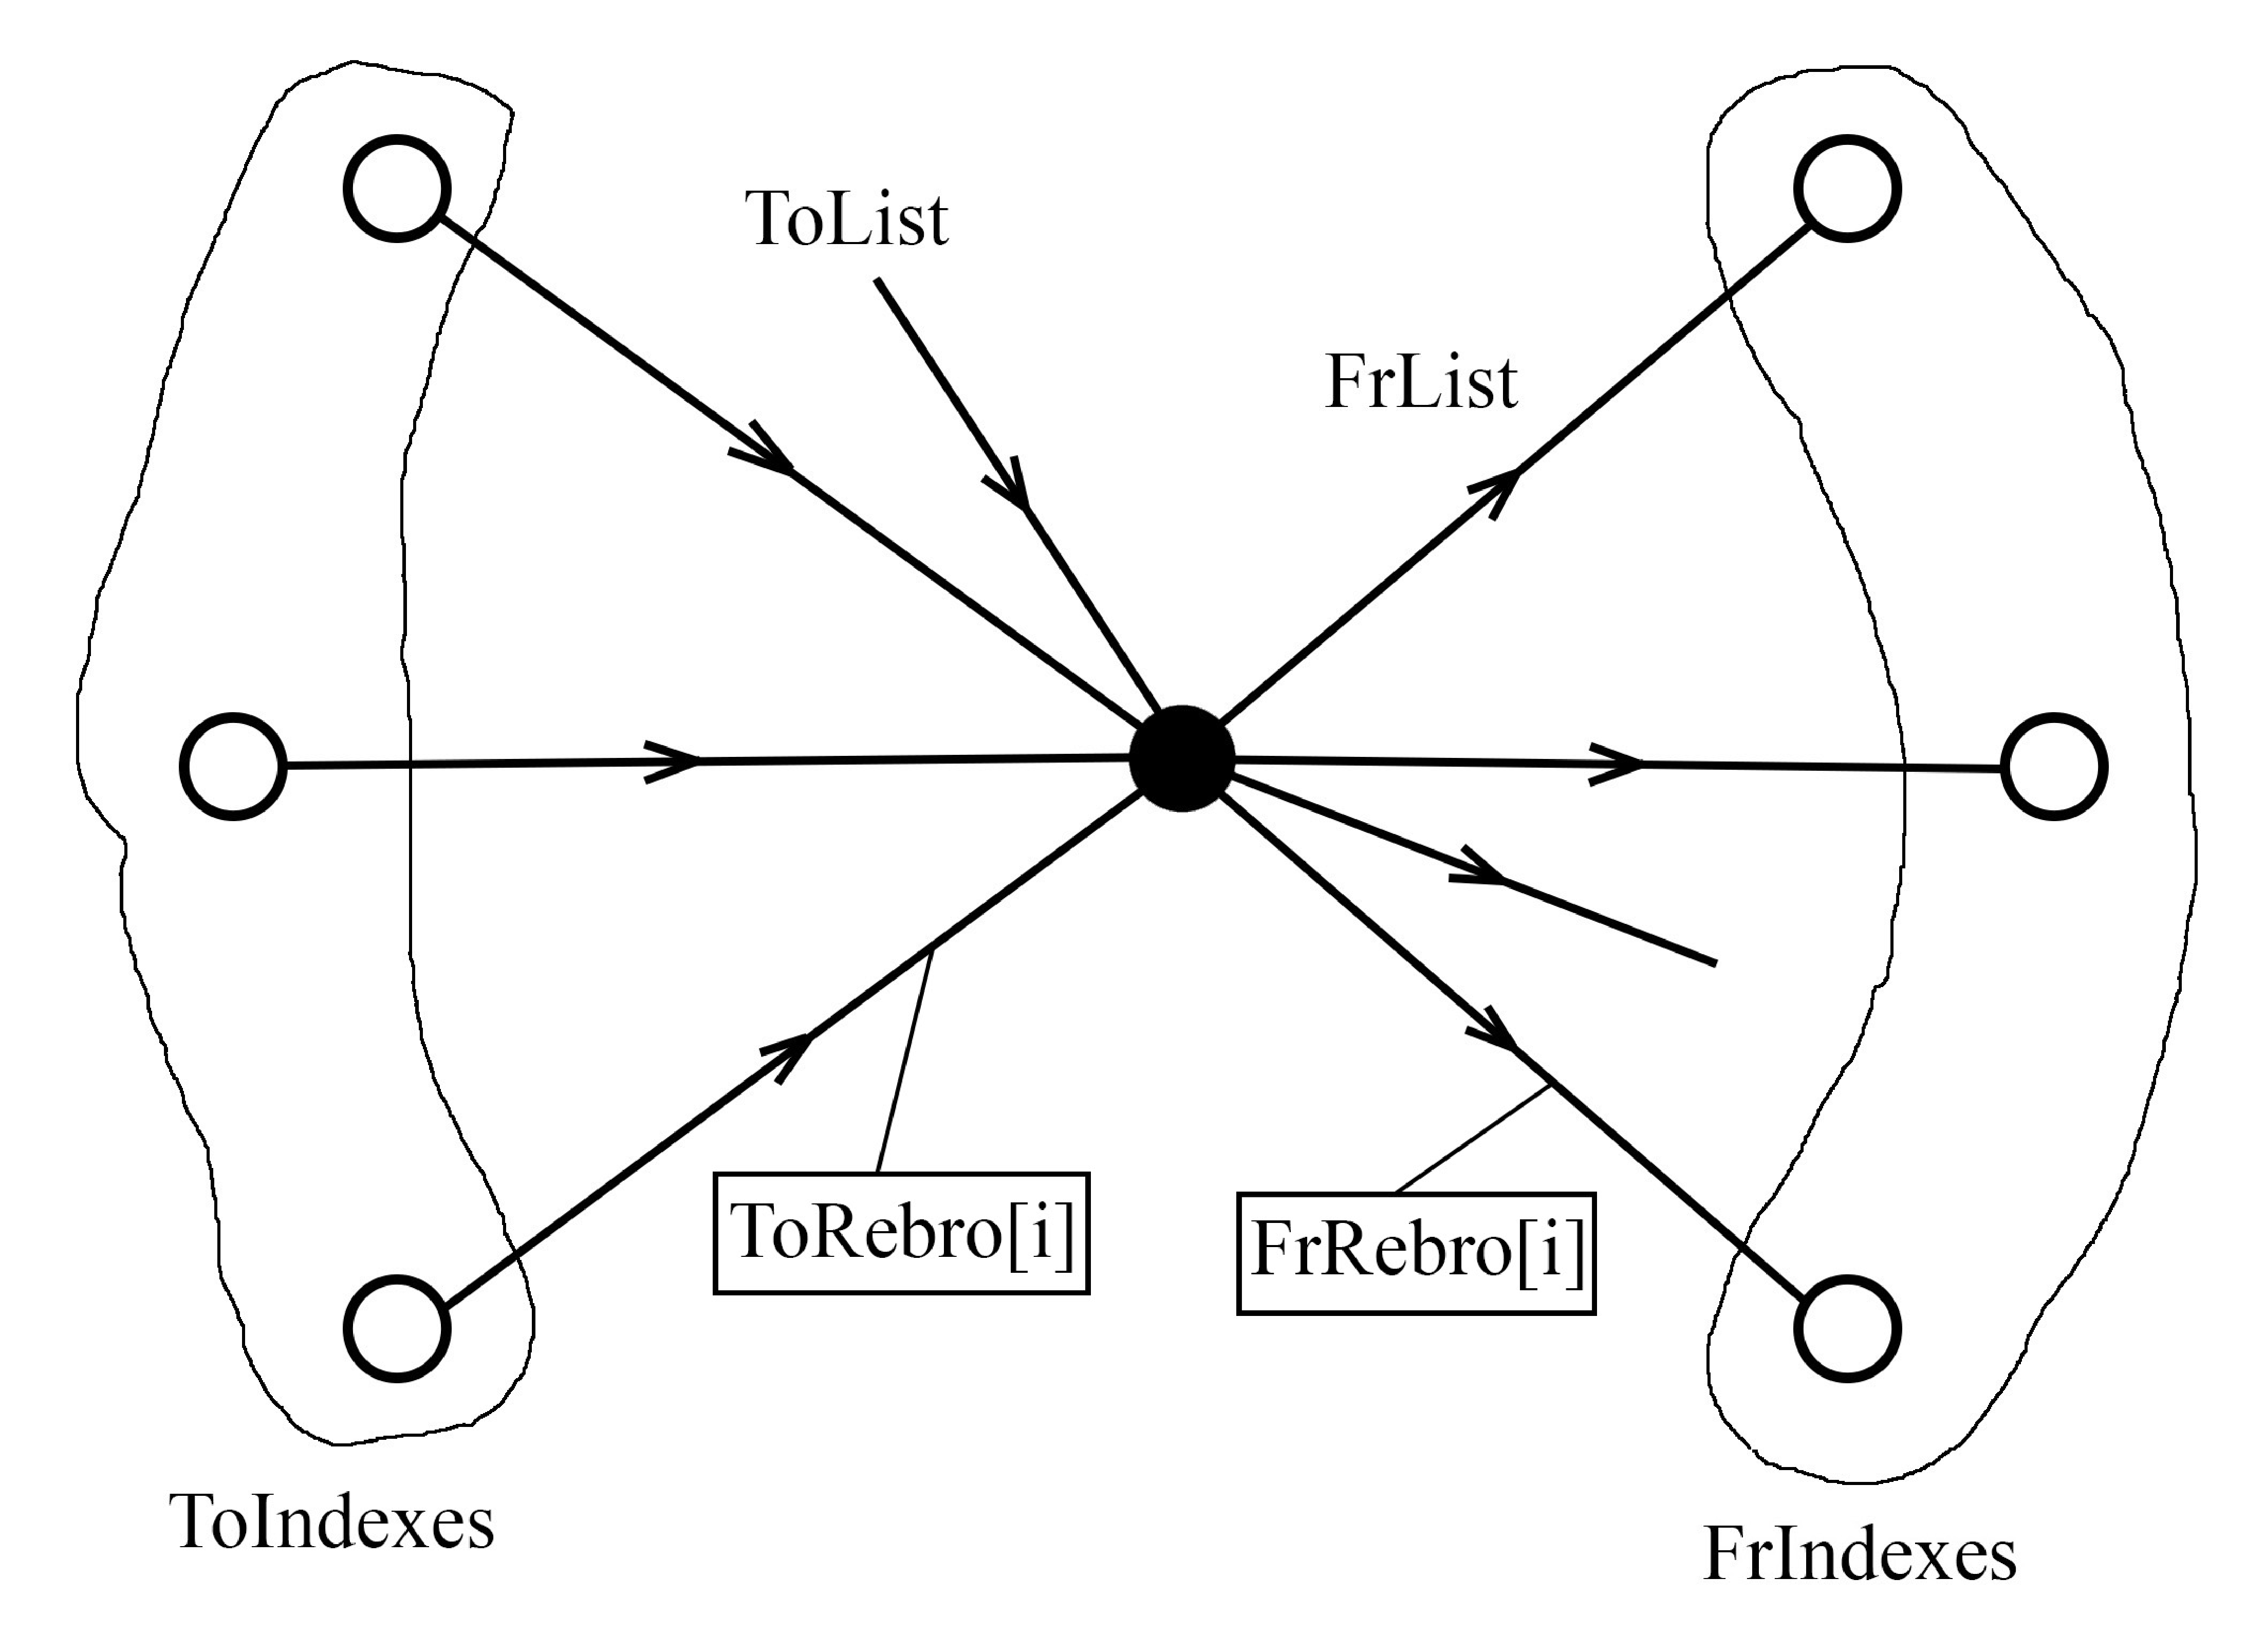
\includegraphics[width=1.0\linewidth]{Uzel_conn.eps}
\caption{\textsc{Схема связей для узла}}\label{fig61}
}
\end{figure}

В процессе анализа топологии расчётной схемы для узла составляются следующие списки:
\begin{enumerate}[topsep=5pt, itemsep=-3pt]
\item ToList --- список входящих в узел рёбер;
\item FrList --- список выходящих из узла рёбер;
\item UzelList --- список, содержащий имена данного узла и всех связанных с ним узлов;
\item ToIndexes --- список, содержащий локальные номера узлов из списка ToList;
\item FrIndexes --- список, содержащий локальные номера узлов из списка FrList,
\end{enumerate}
а также массив cJac глобальных номеров узлов из списка UzelList.

Запишем уравнения сохранения импульса для последних гидравлических связей рёбер, входящих в рассматриваемый узел:
\begin{equation}
\label{formula625}
(A_N^G)_{k_1} \cdot (\Delta(dP_{N-1}^n))_{k_1}+(B_N^G)_{k_1} \cdot (\Delta(dG_N^n))_{k_1} + (C_N^G)_{k_1} \cdot \Delta(dP_u^n)  = (-F_N^G)_{k_1}, 
\end{equation}
где $k_1$ --- номер входящего ребра; $N-1$ --- номер последней расчётной ячейки входящего в узел ребра; $N$ --- номер последней гидравлической связи входящего в узел ребра; $dP_u^n$ --- давление в рассматриваемом узле.

Запишем уравнения сохранения импульса для первых гидравлических связей рёбер, выходящих из рассматриваемого узла:
\begin{equation}
\label{formula626}
(A_0^G)_{k_2} \cdot \Delta(dP_u^n)+(B_0^G)_{k_2} \cdot (\Delta(dG_0^n))_{k_2} + (C_0^G)_{k_2} \cdot (\Delta(dP_0^n))_{k_2}  = (-F_0^G)_{k_2}, 
\end{equation}  
где $k_2$ --- номер выходящего ребра; $0$ --- номер первой ячейки выходящего из узла ребра и номер первой гидравлической связи.

Подставим в уравнения сохранения импульса вместо давлений в ячейках, примыкающих к узлу, их выражения через давления во входном и выходном узлах канала. Тогда для входящих рёбер получим
\begin{align}
\label{formula627}
&(A_N^G)_{k_1} \cdot \left[(S_{N-1}^0)_{k_1} + (S_{N-1}^1)_{k_1} \Delta(dP_{u_{in}}^n)_{k_1} + (S_{N-1}^2)_{k_1} \Delta(dP_u^n)\right]+(B_N^G)_{k_1} \cdot (\Delta(dG_N^n))_{k_1}+\notag ~\\
& + (C_N^G)_{k_1} \cdot \Delta(dP_u^n) = (-F_N^G)_{k_1}, 
\end{align}
а для выходящих рёбер ---
\begin{align}
\label{formula628}
&(A_0^G)_{k_2} \cdot \Delta(dP_u^n)+(B_0^G)_{k_2} \cdot (\Delta(dG_0^n))_{k_2} + \notag ~\\
& + (C_0^G)_{k_2} \cdot \left[(S_0^0)_{k_2} + (S_0^1)_{k_2} \Delta(dP_u^n) + (S_0^2)_{k_2} \Delta(dP_{u_{out}}^n)_{k_2}\right]  = (-F_0^G)_{k_2}, 
\end{align}
где $(dP_{u_{in}}^n)_{k_1}$ --- давление в узле на входе в $k_1$-е входящее ребро, а $(dP_{u_{out}}^n)_{k_2}$ --- давление в узле на выходе из $k_2$-го выходящего ребра. 

Выразим из полученных уравнений расходы в гидравлических связях:
\begin{align}
\label{formula629}
(\Delta(dG_N^n))_{k_1} = \frac{1}{(B_N^G)_{k_1}}\cdot \Big[
(-F_N^G)_{k_1}-(A_N^G)_{k_1}\cdot \big[(S_{N-1}^0)_{k_1} + (S_{N-1}^1)_{k_1} \Delta(dP_{u_{in}}^n)_{k_1} + \notag ~\\
+ (S_{N-1}^2)_{k_1} \Delta(dP_u^n)\big] - (C_N^G)_{k_1} \Delta(dP_u^n)\Big]; \notag ~\\
(\Delta(dG_0^n))_{k_2} = \frac{1}{(B_0^G)_{k_2}}\cdot \Big[(-F_0^G)_{k_2} - (A_0^G)_{k_2} \Delta(dP_u^n) - \notag ~\\
- (C_0^G)_{k_2}\cdot \big[(S_0^0)_{k_2} + (S_0^1)_{k_2} \Delta(dP_u^n) + (S_0^2)_{k_2} \Delta(dP_{u_{out}}^n)_{k_2}\big] \Big].
\end{align}

Раскроем скобки и сгруппируем слагаемые с давлениями в узлах и все остальные. Получим
\begin{align}
\label{formula630}
(\Delta(dG_N^n))_{k_1} = \frac{1}{(B_N^G)_{k_1}}\cdot \Big[[(-F_N^G)_{k_1}-(A_N^G)_{k_1}(S_{N-1}^0)_{k_1}]-(A_N^G)_{k_1}(S_{N-1}^1)_{k_1} \Delta(dP_{u_{in}}^n)_{k_1}-\notag ~\\
-[(A_N^G)_{k_1}(S_{N-1}^2)_{k_1}+(C_N^G)_{k_1}] \Delta(dP_u^n)      \Big]; \notag ~\\
(\Delta(dG_0^n))_{k_2} = \frac{1}{(B_0^G)_{k_2}}\cdot \Big[[(-F_0^G)_{k_2}-(C_0^G)_{k_2}(S_0^0)_{k_2}]-[(A_0^G)_{k_2}+(C_0^G)_{k_2}(S_0^1)_{k_2}]\Delta(dP_u^n) - \notag ~\\
- (C_0^G)_{k_2}(S_0^2)_{k_2} \Delta(dP_{u_{out}}^n)_{k_2} \Big].
\end{align}

Подставим эти расходы в уравнение сохранения массы для узла вида~\eqref{formula518}
\begin{align}
\label{formula631}
\left(A_k^P \right)'\cdot \sum_{j=1}^{K1} \frac{1}{(B_N^G)_j}\cdot \Big[[(-F_N^G)_j-(A_N^G)_j(S_{N-1}^0)_j]-(A_N^G)_j(S_{N-1}^1)_j \Delta(dP_{u_{in}}^n)_j - \notag ~\\
-[(A_N^G)_j(S_{N-1}^2)_j+(C_N^G)_j] \Delta(dP_u^n) \Big] + \left(B_k^P \right)' \cdot \Delta(dP_u^n) + \notag ~\\ 
+ \left(C_k^P \right)'\cdot \sum_{j=1}^{K2} \frac{1}{(B_0^G)_j}\cdot \Big[[(-F_0^G)_j-(C_0^G)_j(S_0^0)_j]-[(A_0^G)_j+(C_0^G)_j(S_0^1)_j]\Delta(dP_u^n) - \notag ~\\
- (C_0^G)_j(S_0^2)_j \Delta(dP_{u_{out}}^n)_j \Big] = -\left(F_k^P \right)',
\end{align}
где $k$ --- номер рассматриваемого узла; $K1$ --- количество входящих в рассматриваемый узел рёбер; $K2$ --- количество выходящих из рассматриваемого узла рёбер.

Выделим из полученного уравнения члены перед давлениями в соседних узлах, перед давлением в данном узле, и свободный член. Тогда будем иметь:
\begin{itemize}[topsep=5pt, itemsep=-3pt]
\item множитель перед давлениями во входящих узлах
\begin{equation}
\label{formula632}
\left(A_k^P \right)_j^{*}=\left(A_k^P \right)' \cdot \frac{1}{(B_N^G)_j}\cdot\left[-(A_N^G)_j(S_{N-1}^1)_j\right];
\end{equation}
\item множитель перед давлениями в выходящих узлах
\begin{equation}
\label{formula633}
\left(C_k^P \right)_j^{*}=\left(C_k^P \right)' \cdot \frac{1}{(B_0^G)_j}\cdot\left[-(C_0^G)_j(S_0^2)_j\right];
\end{equation}
\item множитель перед давлением в рассматриваемом узле
\begin{align}
\label{formula634}
\left(B_k^P \right)^{*}=\left(B_k^P \right)'&+\left(A_k^P \right)'\cdot \sum_{j=1}^{K1} \frac{-1}{(B_N^G)_j}\cdot[(A_N^G)_j(S_{N-1}^2)_j+(C_N^G)_j] + \notag ~\\
&+ \left(C_k^P \right)'\cdot \sum_{j=1}^{K2} \frac{-1}{(B_0^G)_j}\cdot [(A_0^G)_j+(C_0^G)_j(S_0^1)_j];
\end{align}
\item свободный член
\begin{align}
\label{formula635}
\left(F_k^P \right)^{*}=\left(F_k^P \right)'&+\left(A_k^P \right)'\cdot \sum_{j=1}^{K1} \frac{-1}{(B_N^G)_j}\cdot[(F_N^G)_j+(A_N^G)_j(S_{N-1}^0)_j] + \notag ~\\
&+\left(C_k^P \right)'\cdot \sum_{j=1}^{K2} \frac{-1}{(B_0^G)_j}\cdot [(F_0^G)_j+(C_0^G)_j(S_0^0)_j]. 
\end{align}
\end{itemize} 

С использованием сокращённых обозначений~\eqref{formula632} -- \eqref{formula635} окончательно уравнение сохранения массы для узла запишем в виде
\begin{equation}
\label{formula636}
\sum_{j=1}^{K1}\left(A_k^P \right)_j^{*}\cdot\Delta(dP_{u_{in}}^n)_j  + \left(B_k^P \right)^{*} \cdot \Delta(dP_k^n) + \sum_{j=1}^{K2} \left(C_k^P \right)_j^{*}\cdot \Delta(dP_{u_{out}}^n)_j  = -\left(F_k^P \right)^{*}.
\end{equation}

Если записать эти уравнения для всех внутренних узлов схемы, то получится СЛАУ относитель давлений в узлах. Размер матрицы этой СЛАУ будет равен $n\times n$, где $n$ --- общее количество внутренних узлов в схеме. Ненулевыми в каждой строке этой матрицы будут члены, соответствующие тем узлам, с которыми связан узел этой строки, и член, соответствующий самому узлу этой строки. Если решить СЛАУ каким-либо способом, то найдём погрешности для давлений в узлах на $r$-й итерации на текущем шаге по времени.

По найденным погрешностям для давлений в узлах найдём по уравнениям~\eqref{formula623} погрешности для давлений во всех расчётных ячейках всех каналов. Затем по уравнениям метода Ньютона-Рафсона~\eqref{formula55} можно перейти на $(r+1)$-ю итерацию на текущем шаге по времени.

По утверждению автора диссертации \cite{DisserKORSAR} этот метод расчёта поля давления в контуре произвольной топологии, названный им "безытерационным"{}, "превосходит известные классические методы решения полной системы уравнений относительно давлений в расчётных ячейках разветвлённого контура циркуляции более чем на порядок по быстродействию".  
 
Например, в диссертации приводятся результаты сравнения быс\-тро\-дей\-стви\-я пре\-дло\-жен\-но\-го метода относительно метода разреженных матриц библиотеки NAG для условий, когда количество точек ветвления значительно меньше общего количества расчётных ячеек. Показано, что безытерационный метод расчёта поля давления приблизительно в 17 раз превосходит метод разреженных матриц библиотеки NAG, и этот показатель не зависит от количества расчётных ячеек.

Следует, однако, учитывать, что в диссертации метод предлагается для расчёта двухфазных течений по более сложной физической модели по сравнению с заложенной в теплогидравлический код SimInTech, и, кроме того, там не рассматривается использование итерационного метода Ньютона-Рафсона (или какого-либо другого) для определения искомых величин на каждом шаге по времени. Одним словом, вопрос быстродействия метода требует отдельного исследования.    






 




